\documentclass[10pt]{article}
\usepackage[margin=0.75in, top=0.75in, bottom=0.75in]{geometry}
\usepackage{times}
\usepackage{microtype}
\usepackage{enumitem}
\usepackage{hyperref}
\usepackage{graphicx}
\usepackage{tikz}
\usetikzlibrary{arrows.meta,positioning,fit,backgrounds}
\usepackage{titlesec}

\hypersetup{
  colorlinks=true,
  linkcolor=black,
  urlcolor=blue,
  citecolor=black
}

\setlist[itemize]{leftmargin=*,noitemsep,topsep=2pt,parsep=0pt,partopsep=0pt}
\titlespacing*{\section}{0pt}{8pt}{4pt}
\setlength{\parskip}{0pt}
\setlength{\parindent}{0pt}

\begin{document}

\begin{center}
{\Large \textbf{Prompt2Model: Language-Guided Vision Model Factory}}\\
\vspace{4pt}
\textbf{Dev Sanghvi} (ds221)\hspace{10pt}
\textbf{Venkata Sai Aneesh Thatiparti} (vt20)\hspace{10pt}
\textbf{Madhuvani Thatiparti} (mt180)\\
\vspace{2pt}
\end{center}

\vspace{-4pt}
\section*{Motivation}
Modern vision training pipelines require many expert choices (task setup, label mapping, augmentations, model family, hyperparameters, and export format). This creates friction for rapid prototyping and deployment, especially for edge/real-time applications. We propose a \textbf{vision+language} project: a lightweight \textbf{Language-Guided Vision AutoML} system where a user describes the task in natural language (e.g., ``detect helmets in CCTV footage under low light, prioritize speed'') and the system automatically converts this language specification into a constrained training pipeline, trains a small model within a fixed compute budget, and produces an exportable model pack and evaluation report.

\section*{Proposed Project Idea}
\textbf{Goal:} Build a modest-compute ``model factory'' that takes (1) a \textbf{natural language task spec} and (2) a dataset, then outputs (a) a trained vision model and (b) a structured report. The \textbf{vision+language} component is central: language drives \textbf{label resolution}, \textbf{constraint parsing} (latency/size), and \textbf{recipe selection} (augmentations, backbones, training schedule). We focus on a constrained model pool and budgeted tuning to keep the project feasible.

\textbf{Supported MVP tasks (scoped):}
\begin{itemize}
  \item \textbf{Image Classification} and \textbf{Object Detection} (COCO-style). (Optional stretch: instance segmentation.)
  \item A constrained set of backbones (e.g., 2--3 per task) and a strict compute budget.
\end{itemize}

\section*{System Modules, Inputs/Outputs, and Diagram}
\textbf{Inputs:}
\begin{itemize}
  \item Natural language specification: task type, label names/synonyms, constraints (speed vs accuracy), data assumptions.
  \item Dataset: images + labels (classification folders/CSV; detection COCO JSON).
\end{itemize}

\textbf{Outputs:}
\begin{itemize}
  \item Exported model package (e.g., ONNX + preprocessing/postprocessing configs + label map).
  \item Evaluation report: metrics, failure examples, and resource profile (latency/size estimates).
\end{itemize}

\vspace{6pt}
\begin{center}
\resizebox{0.95\textwidth}{!}{%
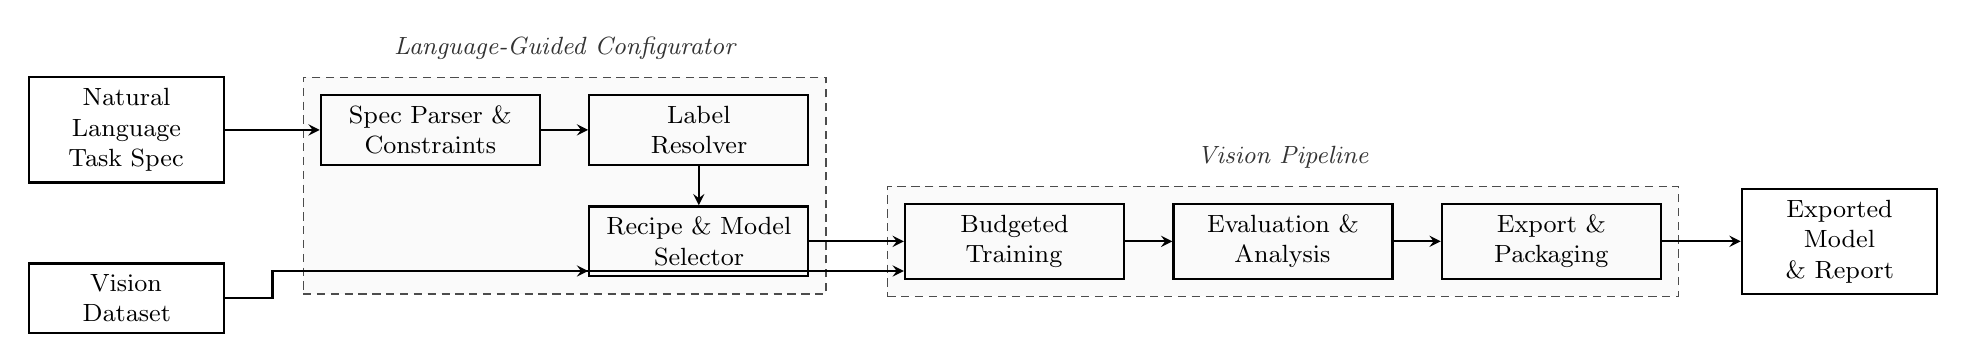
\begin{tikzpicture}[
  >=stealth,
  node distance=6mm and 8mm,
  box/.style={draw=black, thick, align=center, inner sep=4pt, font=\small, minimum height=8mm, text width=2.5cm},
  group/.style={draw=black!70, densely dashed, inner sep=6pt, fill=black!2},
  lbl/.style={font=\small\itshape, text=black!80}
]

% Input Nodes
\node[box, text width=2.2cm] (nl) {Natural Language\\Task Spec};
\node[box, below=1cm of nl, text width=2.2cm] (data) {Vision\\Dataset};

% V+L Module
\node[box, right=1.2cm of nl] (parser) {Spec Parser \&\\Constraints};
\node[box, right=6mm of parser] (resolver) {Label\\Resolver};
\node[box, below=5mm of resolver] (selector) {Recipe \& Model\\Selector};

% Vision Module
\node[box, right=1.2cm of selector] (train) {Budgeted\\Training};
\node[box, right=6mm of train] (eval) {Evaluation \&\\Analysis};
\node[box, right=6mm of eval] (export) {Export \&\\Packaging};

% Output Node
\node[box, right=1cm of export, text width=2.2cm] (out) {Exported Model\\\& Report};

% Groupings
\begin{scope}[on background layer]
  \node[group, fit=(parser) (resolver) (selector)] (vl_group) {};
  \node[lbl, above=1mm of vl_group.north] {Language-Guided Configurator};

  \node[group, fit=(train) (eval) (export)] (vis_group) {};
  \node[lbl, above=1mm of vis_group.north] {Vision Pipeline};
\end{scope}

% Connections
\draw[->, thick] (nl) -- (parser);
\draw[->, thick] (parser) -- (resolver);
\draw[->, thick] (resolver) -- (selector);

\draw[->, thick] (data.east) -- ++(0.6,0) |- (selector.195); % routed to selector
\draw[->, thick] (data.east) -- ++(0.6,0) |- (train.195);    % routed to train

\draw[->, thick] (selector) -- (train);
\draw[->, thick] (train) -- (eval);
\draw[->, thick] (eval) -- (export);

\draw[->, thick] (export) -- (out);

\end{tikzpicture}%
}
\end{center}
\vspace{2pt}

\section*{Evaluation Plan}
We will evaluate both \textbf{vision performance} and the \textbf{language-driven configuration quality}:

\begin{itemize}
  \item \textbf{Model Quality:} Classification accuracy / F1; Detection mAP@0.5 and mAP@[.5:.95] on held-out test splits.
  \item \textbf{Language-to-Config Correctness:} Measure whether parsed labels and constraints match ground-truth intent (manual rubric on 20--30 prompts). Example checks: correct class mapping, correct speed/accuracy preference, correct augmentations triggered (e.g., ``low light'' $\rightarrow$ brightness/contrast).
  \item \textbf{Efficiency Under Budget:} Report training time (GPU-hours), model size, and inference latency proxy (e.g., FPS on a reference machine). Compare: \textbf{(A) language-guided selection} vs \textbf{(B) fixed baseline recipe}.
  \item \textbf{Ablations:} Remove label resolver or constraint extractor and quantify degradation in metrics and/or constraint violations.
\end{itemize}

\section*{Feasibility \& Deliverables}
\textbf{Compute:} Use pretrained backbones and constrained tuning (few trials), enabling modest GPU use.\\
\textbf{Deliverables:} (1) final 4-page report, (2) documented code repo, (3) slides/video demo showing end-to-end: prompt + dataset $\rightarrow$ trained model pack + report.

\vspace{1pt}
\noindent\textbf{Expected Outcome:} A reproducible, end-to-end prototype demonstrating core \textbf{vision+language} concepts: language grounding into a training pipeline, coupled with measurable vision performance and system-level constraints.

\end{document}